\documentclass[12pt]{amsart}
\usepackage[english]{babel}
\usepackage[left=0.75in, right=0.75in, bottom=0.75in, top=0.75in]{geometry}
\usepackage[utf8x]{inputenc}
\usepackage{amsmath,amssymb,amsthm}
\usepackage{enumerate}
\usepackage{graphicx}
\usepackage{booktabs}

\usepackage[table,dvipsnames]{xcolor}
\usepackage{pgf,tikz,tikz-3dplot}
\usetikzlibrary{shapes,arrows,positioning,backgrounds}
\tikzset{%
	goodnode/.style={circle, draw=MidnightBlue!90, thick, fill=gray!40},
	okaynode/.style={circle, draw=Orange!90, thick, fill=gray!40},
	badnode/.style={circle, draw=Red!90, thick, fill=gray!40},
	togood/.style={draw=MidnightBlue, thick,->,>=stealth',shorten >=1pt},
	tookay/.style={draw=Orange, thick,->,>=stealth',shorten >=1pt},
	tobad/.style={draw=Red, thick,->,>=stealth',shorten >=1pt}}

\usepackage{float}

\title{OPER 640 - Stochastic Modeling and Analysis}
\author{B. Hosley}
\date{\today}

\begin{document}
	\maketitle
	\raggedbottom

\section{Description}

% Problem description
% 	Paraphrase project description,
% 	formulate analysis questions of interest to leadership

\subsection{The current situation}

After arriving to the data masked location regeneration efforts have begun 
for all aircraft assigned to the squadron.
Three aircraft are undergoing a final inspection and, pending results of that inspection,
will be cleared to fly by the next ATO cycle.
The remaining nine aircraft are undergoing restoration for flight conditions after travel,
Three will finish each ATO cycle for the next three cycles and, pending need
for additional unplanned maintenance, will also be cleared for operation.

\subsection{Purpose of this report}

The purpose of this report is to provide the technical background requested by leadership
supporting the recommendations provided in a previous report.
To this end it will provide information regarding the expected numbers of fully mission 
capable aircraft available for sortie generation, and how these estimations were determined.
Provided the intent is met, it will provide greater confidence in the information
provided to decision makers to make and take more informed courses of action.

\subsection{Initial inquiries}

First, we will examine the expected time it will take, starting from the 
current situation, for the squadron to return to sortie generating capable.
Second, we will examine the expected long term availability of aircraft
if the current operational conditions persist.
Finally, we will examine the effects of changes to current operations, 
to provide the information necessary to evaluate which of those changes 
will have the greatest return on investment.


\section{Modeling the Situation}

\subsection{Model Specifications}

Based on the information provided, this system will lend itself well to being modeled 
by a discrete-time Markov chain.
This system will be 

\(\{X_n : n\geq0\}\)

\(X_n = \{X_n^1,X_n^2,X_n^3,X_n^4,X_n^5\}\)
Where \(X_n^i\) represents the number of aircraft in state \(i\) at time \(n\)
the states are classified as


\begin{tabular}{rl}
	\toprule
	\(i\) & \textit{State Description} \\
	\midrule
	1 & Fully mission capable \\
	2 & In the front shop for inspection or minor repair \\
	3 & First ATO cycle in backshop \\
	4 & Second ATO cycle in backshop \\
	5 & Last ATO cycle in backshop \\
	\bottomrule
\end{tabular}

The state space, or the list of every possible configuration of this model

\(\sum_{i=1}^{5}X_n^i = 12\)

The state space will not be further enumerated here, as it can be seen

\(\left( \hspace{-0.4em} \binom{n}{k} \hspace{-0.4em} \right) \)

%DTMC model formulation (Lesson2 slide 18 (with single entity transition diagram))


% Define the state space S as the set of all possible outcomes for Xn


% Verify the Markov Property is satisfied.


% Verify Time-Homogeneity


% Construct the Transition Probability Matrix. Or specify probability function p_ij.
% As needed:
% 	Formulate state transition function (X_n+1 as a function of X_n)
% 	Draw a Transition Diagram.
% 	Define a cost or reward function.

Figure \ref{DTMC} shows the state-cycle of an individual aircraft.

\begin{figure}[H]
	\centering
	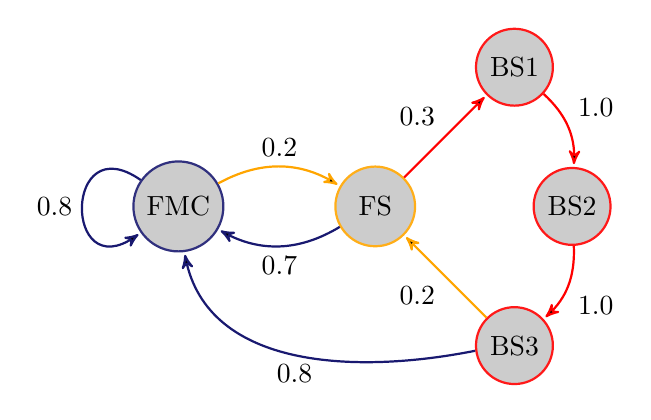
\begin{tikzpicture}[node distance=2.5cm]		
		\node[goodnode] (FMC) {FMC};
		\node[okaynode] (FS) [right of=FMC] {\(\ \)FS\(\ \)};
		\node[badnode] (BS1) [above right of=FS] {BS1};
		\node[badnode] (BS2) [right of=FS] {BS2};
		\node[badnode] (BS3) [below right of=FS] {BS3};
		
		\path[togood] (FMC) 	edge [loop left, min distance=12mm, out=145, in=215]  node [left] 	{\(0.8\)} (FMC);
		\path[togood] (FS)  	edge [bend left]  node [below] 	{\(0.7\)} (FMC);
		\path[togood] (BS3) 	edge [bend left, in=120]  node [below] 	{\(0.8\)} (FMC);
		
		\path[tookay] (FMC) 	edge [bend left]  node [above] 	{\(0.2\)} (FS);
		\path[tookay] (BS3) 	edge []  node [below left] 	{\(0.2\)} (FS);
		
		\path[tobad]  (FS) 		edge []  node [above left] 	{\(0.3\)} (BS1);
		\path[tobad]  (BS1) 	edge [bend left=25]  node [above right] 	{\(1.0\)} (BS2);
		\path[tobad]  (BS2) 	edge [bend left=25]  node [below right] 	{\(1.0\)} (BS3);
	\end{tikzpicture}
	\caption{Single Entity DTMC.}
	\label{DTMC}
\end{figure}



\section{Baseline Analysis}

% Baseline analysis - primary analysis questions
% 	How often will the squadron be able to achieve mission success, meeting 8-orbit mission requirements
% 	How long will it take for the squadron become FMC >= 8 aircraft
% 	What is the long-term sortie generation rate?
% 	What is the long-term mission capable aircraft availability rate?

\section{Exploratory Analysis}

% Sensitivity (excursion) analyses - the what-if questions, 
% 	explore possible solutions by modifying parameter values

\section{Conclusions and Recommendations}

% Conclusions and recommendations


\end{document}